\section{API Usage}
\begin{figure}
    \centering
    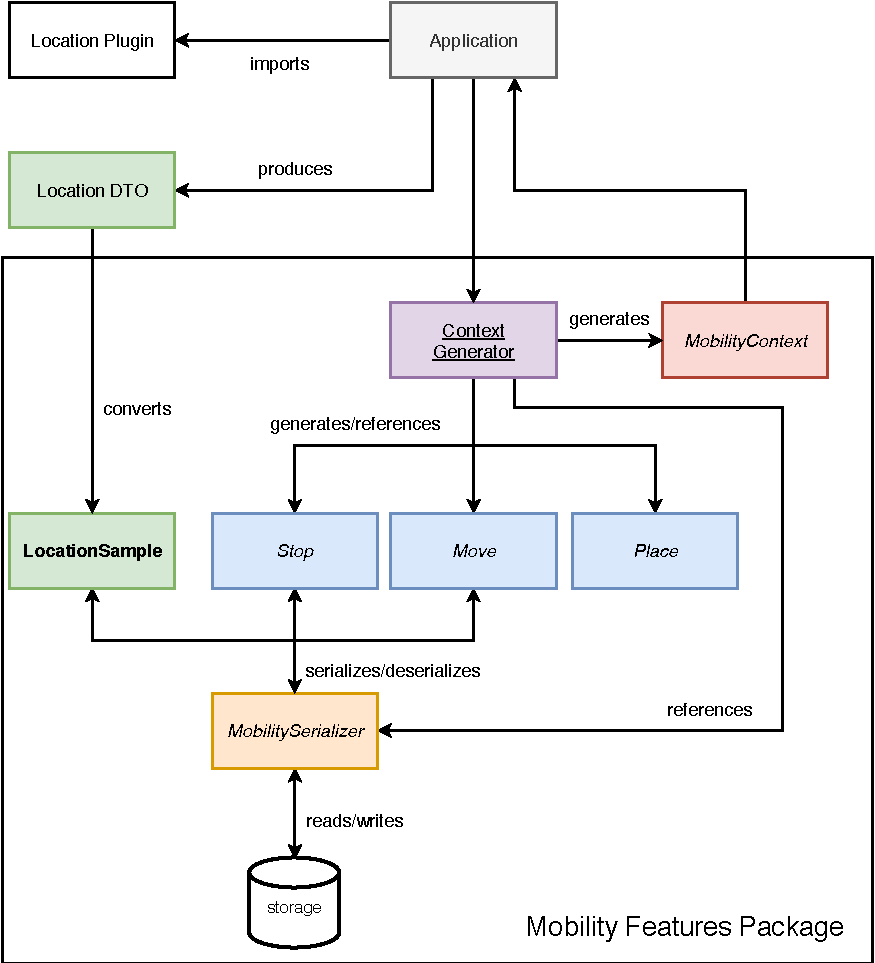
\includegraphics[width=\textwidth]{images/diagrams/api-diagram.pdf}
    \caption{The components making up the API in which the components highlighted in bold are public facing and those in italics are private.}
    \label{fig:api-diagram}
\end{figure}

\subsection{Computing Intermediate Features}
DATA PREPROC

\subsection{Serialization}
A serializer can be instantiated for in a desktop environment using the \verb|File| class from the built-in package \verb|dart:io| as follows:
\begin{minted}{dart}
    import 'dart:io';
    import 'package:mobility_features/mobility_features_lib.dart';
    ...
    Serializer<Stop> stopSerializer = Serializer(new File(FILENAME));
\end{minted}

In a mobile environment the \verb|path_provider| package is used to get the Documents directory, from which a File object is then created.

\begin{minted}{dart}
    import 'dart:io';
    import 'package:path_provider/path_provider.dart';
    import 'package:mobility_features/mobility_features_lib.dart';
    ...
    String path = (await getApplicationDocumentsDirectory()).path;
    Serializer<Stop> stopSerializer = Serializer(new File(path));
\end{minted}

\subsection{Computing Mobility Context(s)}
Create a single Mobility Context without prior Context:

\begin{minted}{dart}
    DateTime today = DateTime.now().midnight;
    DataPreprocessor dp = DataPreprocessor(today);

    List<SingleLocationPoint> points = await _pointSerializer.load();
    List<Stop> stops = dp.findStops(points);
    List<Move> moves = dp.findMoves(points, stops);
    List<Place> places = dp.findPlaces(stops);
    
    MobilityContext mc = MobilityContext(today, stops, places, moves);
\end{minted}

This works for a single day of data, and does not require the user to save previous Stops and Moves. However, the Routine Index cannot be evaluated without using prior contexts. 

% Using prior contexts is much more involved, and will look like the following:

% \begin{minted}{dart}
%     DateTime today = DateTime.now().midnight;
%     DataPreprocessor dp = DataPreprocessor(today);
%     List<Stop> stopsOld = await _stopSerializer.load();
%     List<Move> movesOld = await _moveSerializer.load();
    
%     List<SingleLocationPoint> pointsToday = await _pointSerializer.load();
%     List<Stop> stopsToday = dp.findStops(pointsToday);
%     List<Move> movesToday = dp.findMoves(pointsToday, stopsToday);
%     List<Place> places = dp.findPlaces(stops);
    
%     MobilityContext mc = MobilityContext(today, stops, places, moves);
% \end{minted}